% !TEX root = Eco-Model.tex
\section{Problem Background} % (fold)
\label{sec:problem_background}

\subsection{Cloud Manufacturing Ecosystem} % (fold)
\label{sub:cloud_manufacturing_ecosystem}
As an application of Networked Manufacturing, Cloud Manufacturing proposed by ...

(problems background to form the ecosystem)

Combined with the problem background and other scholars' previous work, we proposed an improved framework that suits for Cloud Manufacturing environment as shown in \autoref{fig:structure}.
\begin{figure}[htbp]
\centering
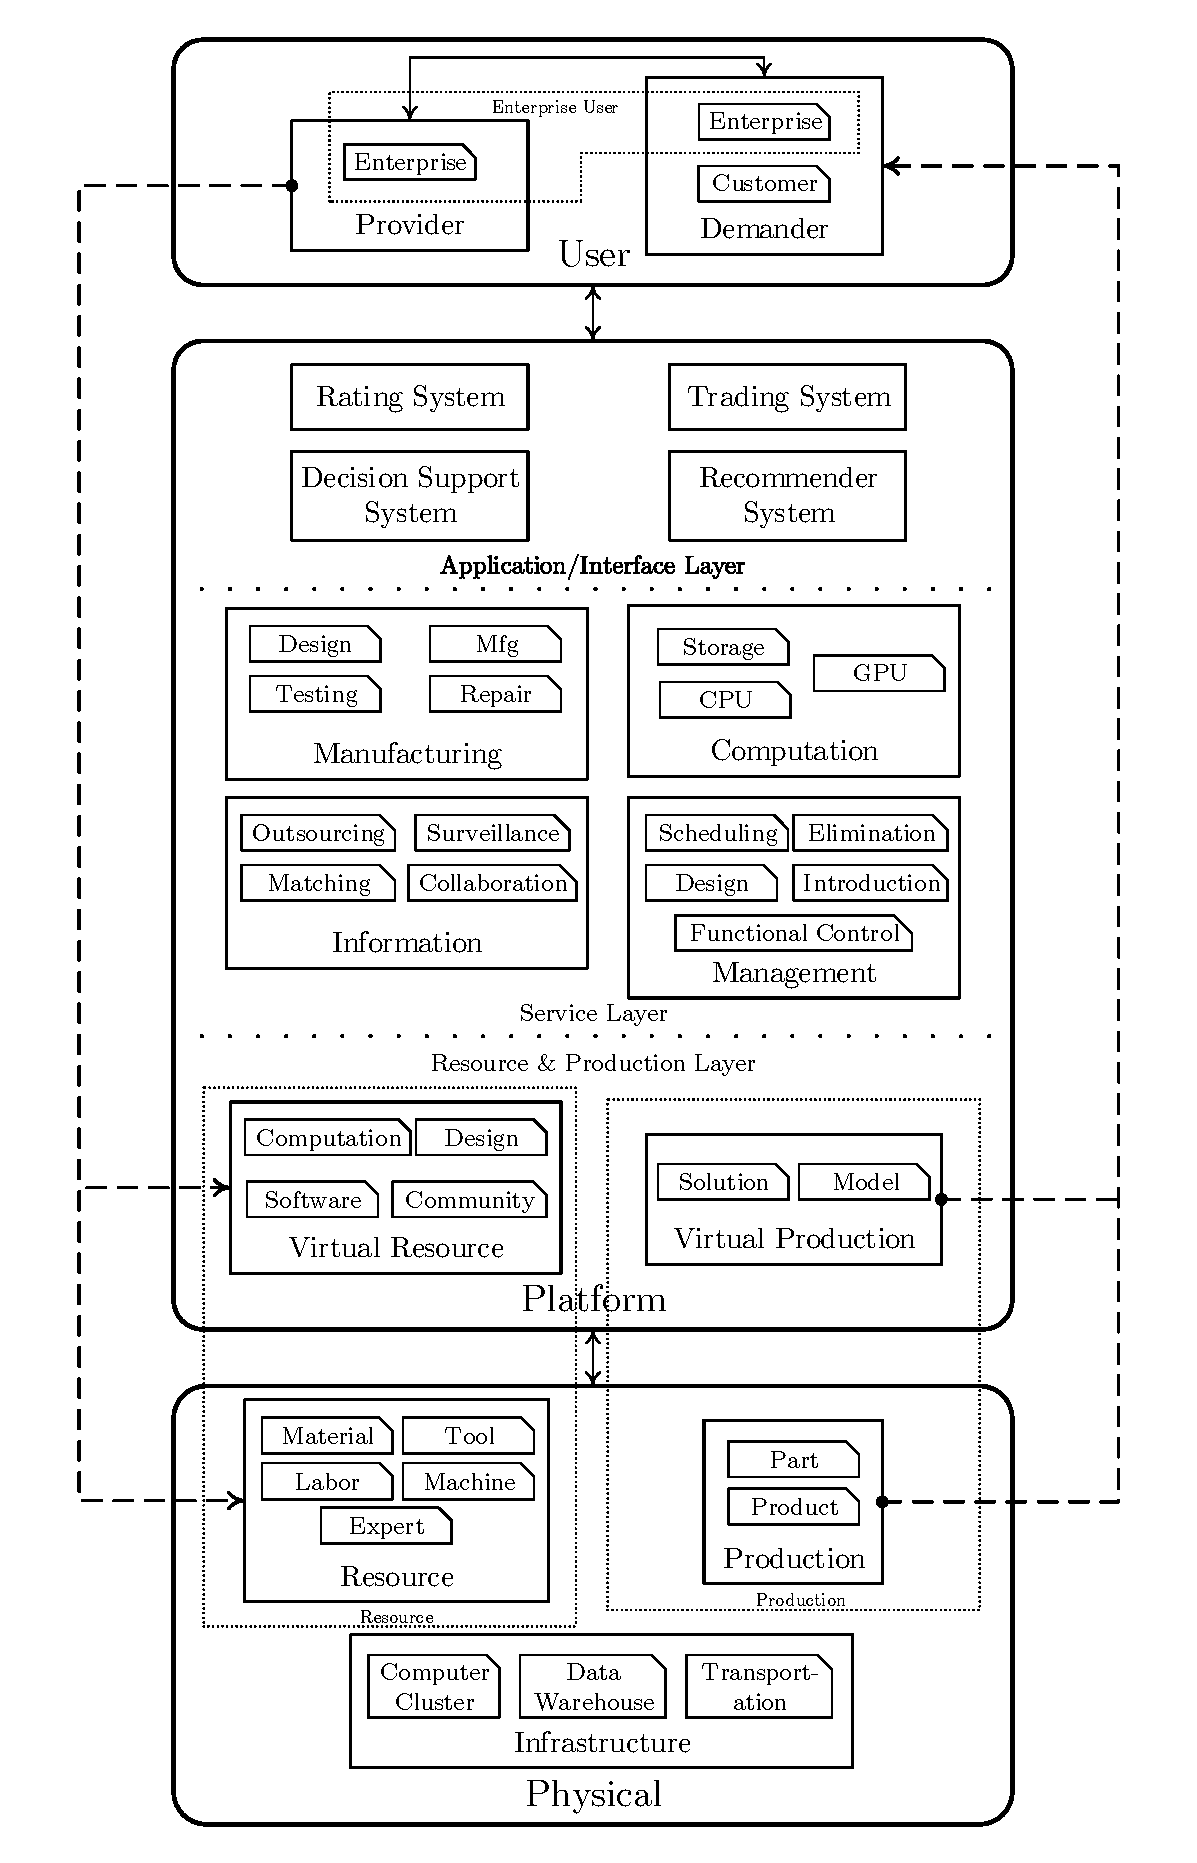
\includegraphics[scale = .6, trim = 0 15 0 35]{Cloud_Mfg_Structure.pdf}
\caption{Cloud Manufacturing Architecture with Main Flows}
\label{fig:structure}
\end{figure}

The architecture of Cloud Manufacturing is mainly composed of three parts, namely, \begin{inparaenum}[1)]
\item User,
\item Platform and
\item Physical Base
\end{inparaenum}, that are connected by material or information flows. A simple version of conception for Cloud Manufacturing architecture we study here can be described as follows:
\begin{compactdesc}
\item [User] part describes the main roles in the Cloud Manufacturing environment like manufacturing service provider and manufacturing service demander, whome can be called as provider and demander for short respectively, from the functional point of view. Meanwhile, these roles can also be classified into enterprise user and customer, from the practical point of view. Both functional and practical are important perspective for later analysis in following sections. 
\item [Platform] part consists of 3 main layers namely \begin{inparaenum}[1)]
\item Application/Interface Layer,
\item Service Layer and 
\item Resource \& Production Layer
\end{inparaenum}.
Service is the core idea of Cloud Manufacturing, so Service Layer is the core of the Cloud Manufacturing platform. With the help of related technology in servitization, manufacturing resource and production can be encapsulated into services, then these services can be acquired by users with the well designed applications or interfaces.
\item [Physical Base] part includes the basic infrastructure, resource and production. It's worth mentioning that part of resources and production can even be virtualized with some services the platform provides.
\end{compactdesc}
 
\begin{figure}[htbp]
\centering
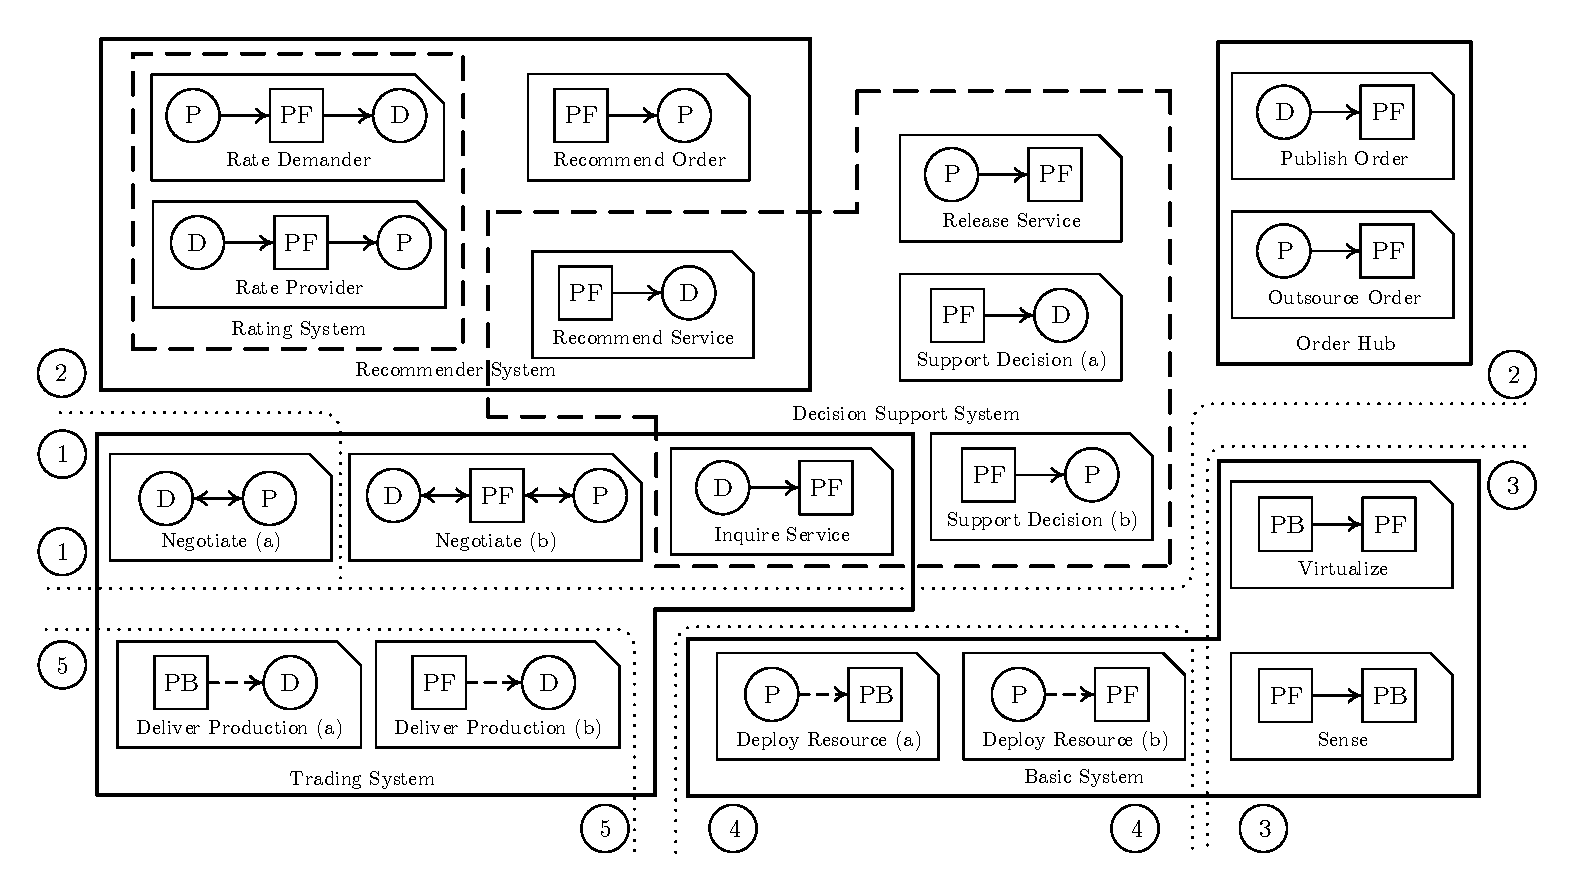
\includegraphics[scale = .6, trim = 0 15 0 10]{supplementary.pdf}
\caption{Supplementay Illustration for \autoref{fig:structure}}
\label{fig:supplementary}
\end{figure}

With the supplementary illustration of \autoref{fig:supplementary}, which categorizes the main applications in Cloud Manufacturing environment with the forementioned flows that marked by circled number (i.e. \textcircled{\small{1}}) and corresponding to the same symbol in \autoref{fig:structure}, we can simply describe the main activities within the Cloud Manufacturing system. In \autoref{fig:supplementary}, we denote provider, demander, platform and physical base as \textbf{P}, \textbf{D}, \textbf{PF} and \textbf{PB} respectively. The overlap among application districts implies the complexity of the system, so that we will analyse these applications coordinately from a system view.

Modular approaches are widely used to decompose a complex system into smaller subsystems according to their functions. For example, Yang and Li (2011) divided a cloud manufacturing services management and control platform into seven functional modules such as system management module, production management module and so on

\subsubsection{Enterprise Business Mode}

\subsubsection{Resource Sharing Mechanism}

\subsubsection{Ecosystem Adjustment}

% subsection cloud_manufacturing_ecosystem (end)

\subsection{Main Copmlexity Concepts} % (fold)
\label{sub:main_copmlexity_concepts}

\subsubsection{Self-organization}

\subsubsection{Emergence}

\subsubsection{Co-evolution}

\subsubsection{Adaption}
% subsection main_copmlexity_concepts (end)

\subsection{Ecosystem Evolvement} % (fold)
\label{sub:ecosystem_evolvement}

% subsection ecosystem_evolvement (end)

\subsection{Optimal Guidance} % (fold)
\label{sub:optimal_guidance}

% subsection optimal_guidance (end)
% section problem_background (end)